% !TEX root = ../00_tcc.tex

\begin{figure}[h]
	\centering
	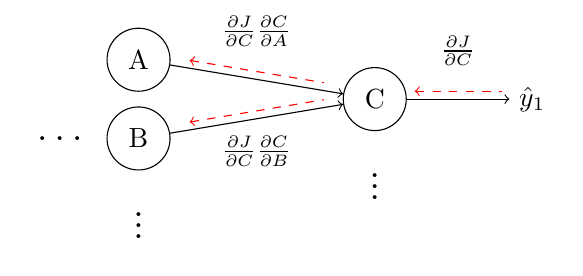
\begin{tikzpicture}
		\tikzstyle{neuron}=[circle, draw=black, minimum size = 8mm]

		\node[]       (lay)  at  (-1,0.5)  {\Large$\dots$};

		\node[neuron] (lay21)  at  (0,1.5)   {A};
		\node[neuron] (lay22)  at  (0,0.5)   {B};
		\node[]       (lay23)  at  (0,-0.5)  {\Large$\vdots$};

		\node[neuron] (out1)    at  (3,1)   {C};
		\node[]                 at  (3,0)   {\Large$\vdots$};

		\draw[->]  (lay21)  --  (out1)  ;
		\draw[->]  (lay22)  --  (out1)  ;
		\node[]       (resul1)  at  (5,1)   {$\hat{y}_1$};
		\draw[->]  (out1)   --  (resul1)  ;


		\begin{scope}[transform canvas={yshift=1mm}]
			\draw[<-, red, shorten >=1mm,  shorten <=1mm,   dashed]  (out1)  --
				(resul1) node[pos=0.5,above=2mm, black] {\small $\frac{\partial J}{\partial C}$};
			\draw[<-, red, shorten >=2.5mm,shorten <=2.5mm, dashed]  (lay21) --
				(out1) (resul1) node[pos=0.5,above=2mm, black] {\small $\frac{\partial J}{\partial C}\frac{\partial C}{\partial A}$};
			\draw[<-, red, shorten >=2.5mm,shorten <=2.5mm, dashed]  (lay22) --
				(out1) (resul1) node[pos=0.5,below=2mm, black] {\small $\frac{\partial J}{\partial C}\frac{\partial C}{\partial B}$};
		\end{scope}

	\end{tikzpicture}
	\caption{\acrshort{bp} através da regra da cadeia. Fonte: própria.}\label{tikz:bp}
\end{figure}
